\section{Auswertung}
\label{sec:Auswertung}
\subsection{Winkelrichtgröße}
Die Winkelrichtgröße wird durch die Formel
\begin{equation}
  D = \frac{F \cdot r}{\phi}
\end{equation}
bestimmt. Die verwendeten Werte sind in Tabelle \ref{tab:winkelrichtgr} angegeben.
\begin{table}
  \centering
  \caption{Messdaten zur Bestimmung der Winkelrichtgröße D}
  \label{tab:winkelrichtgr}
  \begin{tabular}{c c c c}
    \toprule
    $F/N$ & $\phi /^{\circ}$ & $r/m$ & $D/Nm$ \\
    \midrule
    0,1  &  30 & 0,1 & 0,000333 \\
    0,26 &  60 & 0,1 & 0,000433 \\
    0,41 &  90 & 0,1 & 0,000456 \\
    0,56 & 120 & 0,1 & 0,000467 \\
    0,72 & 150 & 0,1 & 0,000480 \\
    0,85 & 180 & 0,1 & 0,000472 \\
    0,48 & 180 & 0,2 & 0,000533 \\
    0,55 & 240 & 0,2 & 0,000458 \\
    0,63 & 270 & 0,2 & 0,000467 \\
    0,69 & 300 & 0,2 & 0,000460 \\
    \bottomrule
  \end{tabular}
\end{table}
\\Sowohl der Mittelwert, als auch die Standardabweichung wurden mit Python bestimmt. Daraus ergibt sich der
gemittelte Wert
\begin{align*}
    D = (0{,}000456 \pm 0{,}000048)\,\mathrm{Nm} .
\end{align*}

\subsection{Eigenträgheitsmoment}
 \begin{figure}
   \centering
   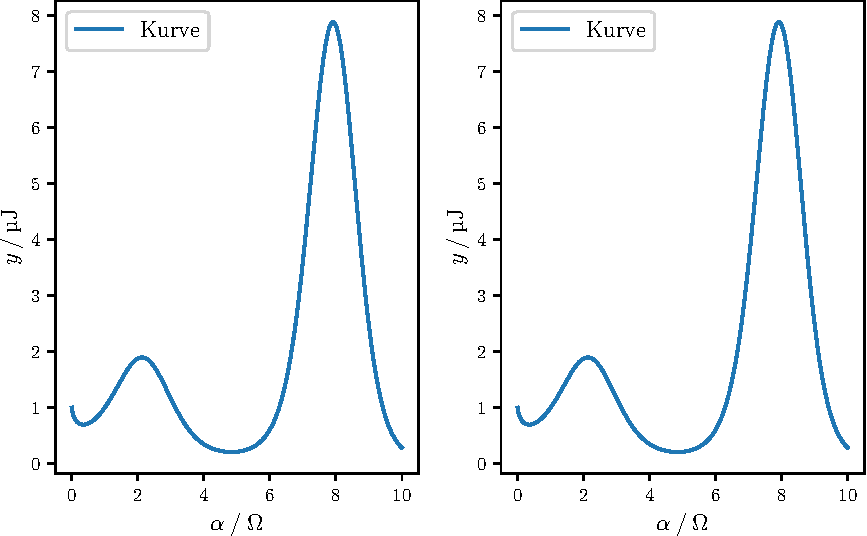
\includegraphics{plot.pdf}
   \caption{Plot.}
   \label{fig:plot}
 \end{figure}

\subsection{Trägheitsmoment des Zylinders}
\subsubsection{Theoretische Werte}

\subsubsection{Experimentelle Werte}
Der Zylinder wird auf der Drillachse um den Winkel $\phi_{Zyl} = 90^{\circ}$ ausgelenkt und die Zeit
nach fünf Schwingungen gestoppt.
Durch teilen der Zeitmessungen $Z_{Zyl}$ durch fünf ergeben sich die Schwingungsdauern $T_{Zyl}$. 
Diese sind in Tabelle \ref{tab:T_Zyl} zu finden.
\begin{table}
  \centering
  \caption{Messdaten der Schwingungsdauer des Zylinders}
  \label{tab:T_Zyl}
  \begin{tabular}{c c}
    \toprule
    $Z_{Zyl}/s$ & $T_{Zyl}/s$ \\
    \midrule
    3,94 & 0,79 \\
    3,75 & 0,75 \\
    4,16 & 0,83 \\
    5,78 & 1,16 \\
    3,69 & 0,74 \\
    3,97 & 0,79 \\
    3,85 & 0,77 \\
    3,84 & 0,77 \\
    4,12 & 0,82 \\
    3,88 & 0,78 \\
    \bottomrule
  \end{tabular}
\end{table}
\\
Der Mittelwert und die Abweichung wurden wieder mit Python berechnet.
Aus den Daten ergibt sich
\begin{align*}
  T_{Zyl} = (0{,}82 \pm 0{,}12)\, \mathrm{s} .
\end{align*}

\subsection{Trägheitsmoment der Kugel}
\subsubsection{Theoretische Werte}

\subsubsection{Experimentelle Werte}
Die Kugel wird auf der Drillachse um $\phi = 90^{\circ}$ ausgelenkt und die Zeit nach drei
Schwingungen gestoppt. Die Schwingungsdauern $T_{Kugel}$ erhält man durch teilen der Zeitmessungen
$Z_{Kugel}$ durch drei. Die Zeitmessungen und berechneten Schwingungsdauern sind in
Tabelle \ref{tab:T_Kugel} zu finden.
\begin{table}
  \centering
  \caption{Messdaten der Schwingungsdauer der Kugel}
  \label{tab:T_Kugel}
  \begin{tabular}{c c}
    \toprule
    $Z_{Kugel}/s$ & $T_{Kugel}/s$ \\
    \midrule
    5,94 & 1,98 \\
    5,71 & 1,90 \\
    5,62 & 1,87 \\
    5,47 & 1,82 \\
    5,63 & 1,88 \\
    5,47 & 1,82 \\
    5,75 & 1,92 \\
    5,47 & 1,82 \\
    5,66 & 1,89 \\
    5,57 & 1,86 \\
    \bottomrule
  \end{tabular}
\end{table}
\\
Der Mittelwert und die Abweichug wurden mit Hilfe von Python bestimmt. Aus den Werten erhält man
\begin{equation}
  T_{Kugel} = (1{,}88 \pm 0{,}05)\, \mathrm{s} .
\end{equation}

\subsection{Trägheitsmoment der Puppe in Körperhaltung 1}
\subsubsection{Theoretische Werte}

\subsubsection{Experimentelle Werte}
Die Puppe wird in der ersten Körperhaltung um $\phi = 90^{\circ}$ ausgelenkt und die Zeit $Z_{K1}$ nach drei
Schwingungen gemessen. Die Schwingungsdauern $T_{K1}$ erhält man durch drei teilen. Die Zeitmessungen und
Schwingunsdauern sind in Tabelle \ref{tab:Koerper1} angegeben.
\begin{table}
  \centering
  \caption{Messdaten der Schwingunsdauer des Körpers in der ersten Position}
  \label{tab:Koerper1}
  \begin{tabular}{c c}
    \toprule
    $Z_{K1}/s$ & $T_{K1}/s$ \\
    \midrule
    2,75 & 0,92 \\
    2,66 & 0,89 \\
    2,66 & 0,89 \\
    2,90 & 0,97 \\
    3,16 & 1,05 \\
    2,56 & 0,85 \\
    2,47 & 0,82 \\
    2,75 & 0,92 \\
    2,53 & 0,84 \\
    2,78 & 0,93 \\
    \bottomrule
  \end{tabular}
\end{table}
\\
Mit Hilfe von Python lässt sich der Mittelwert und die Abweichung bestimmen. Aus den Messdaten
erhält man
\begin{align*}
  T_{K1} = (0{,}91 \pm 0{,}06)\, \mathrm{s} .
\end{align*}
\subsection{Trägheitsmoment der Puppe in Körperhaltung 2}
\subsubsection{Theoretische Werte}

\subsubsection{Experimentelle Werte}
Die Puppe wurde in der zweiten Körperhaltung um $\phi = 90^{\circ}$ ausgelenkt und die Zeit $Z_{K2}$
wurde nach drei Schwingungen gestoppt. Die Schwingungsdauer $T_{K2}$ wird durch teilen von $Z_{K2}$
durch drei. Die Zeitmessungen und Schwingungdsdauern sind in Tabelle\ref{tab:Koerper2} zu finden.
\begin{table}
  \centering
  \caption{Messdaten der Schwingunsdauer des Körpers in der zweiten Position}
  \label{tab:Koerper2}
  \begin{tabular}{c c}
    \toprule
    $Z_{K2}/s$ & $T_{K2}/s$ \\
    \midrule
    1,91 & 0,64 \\
    1,75 & 0,58 \\
    1,75 & 0,58 \\
    1,84 & 0,61 \\
    1,68 & 0,56 \\
    1,84 & 0,61 \\
    1,81 & 0,60 \\
    1,66 & 0,55 \\
    1,84 & 0,61 \\
    1,81 & 0,60 \\
    \bottomrule
  \end{tabular}
\end{table}
\\
Sowohl der Mittelwert, als auch die Standarabweichung wurde mit Python bestimmt.
\begin{align*}
  T_{K2} = (0{,}59 \pm 0{,}03)\, \mathrm{s} .
\end{align*}

Siehe \autoref{fig:plot}!
